\begin{frame}{Review paper - Chapter 4 - Methods}
\vfill
\centering
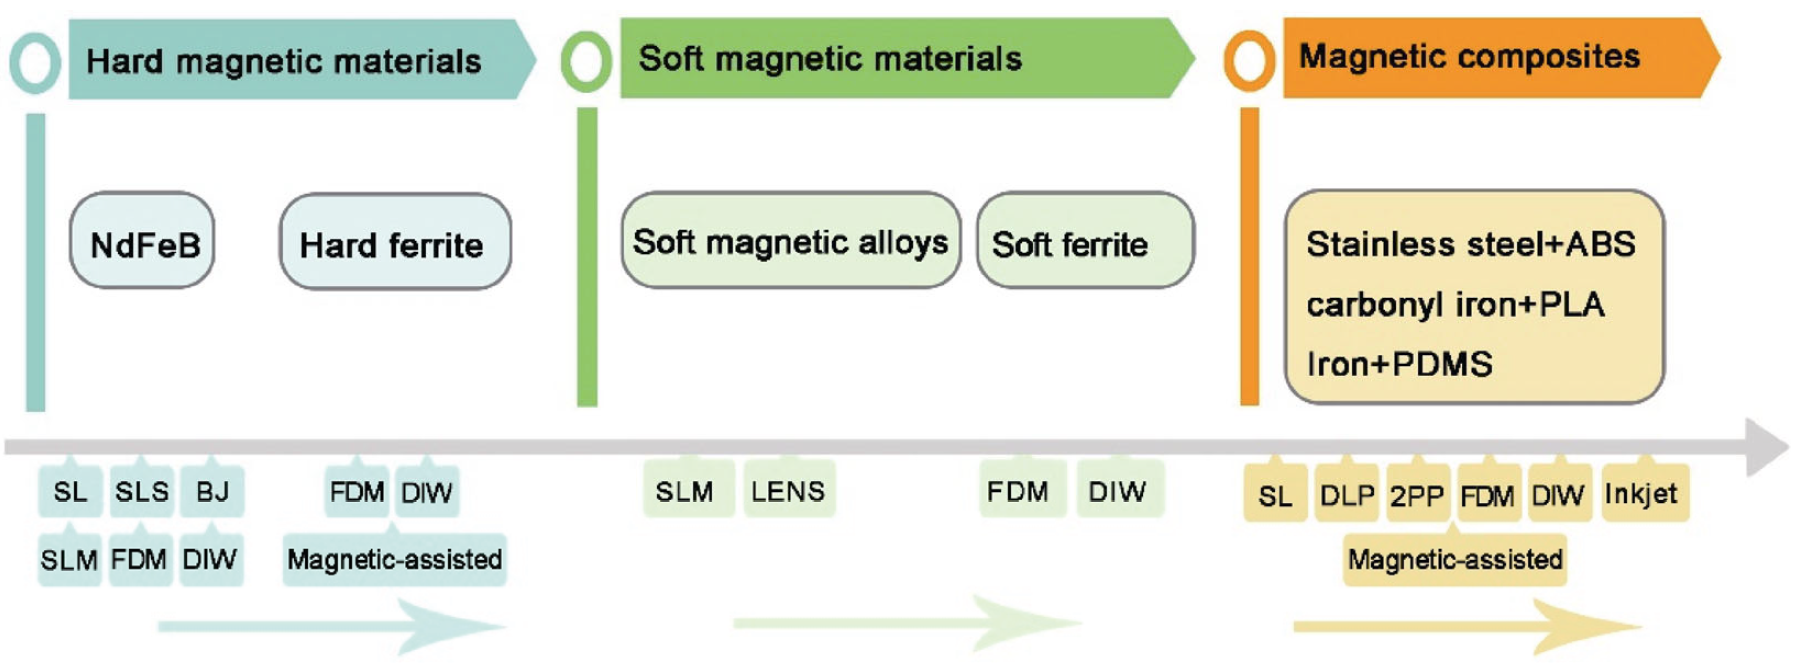
\includegraphics[width=1\textwidth]{images/types_of_AM_magnetic_methods.png}
\vfill

\end{frame}

\begin{frame}{Review paper - Chapter 5 - Applications}
\vfill
\centering
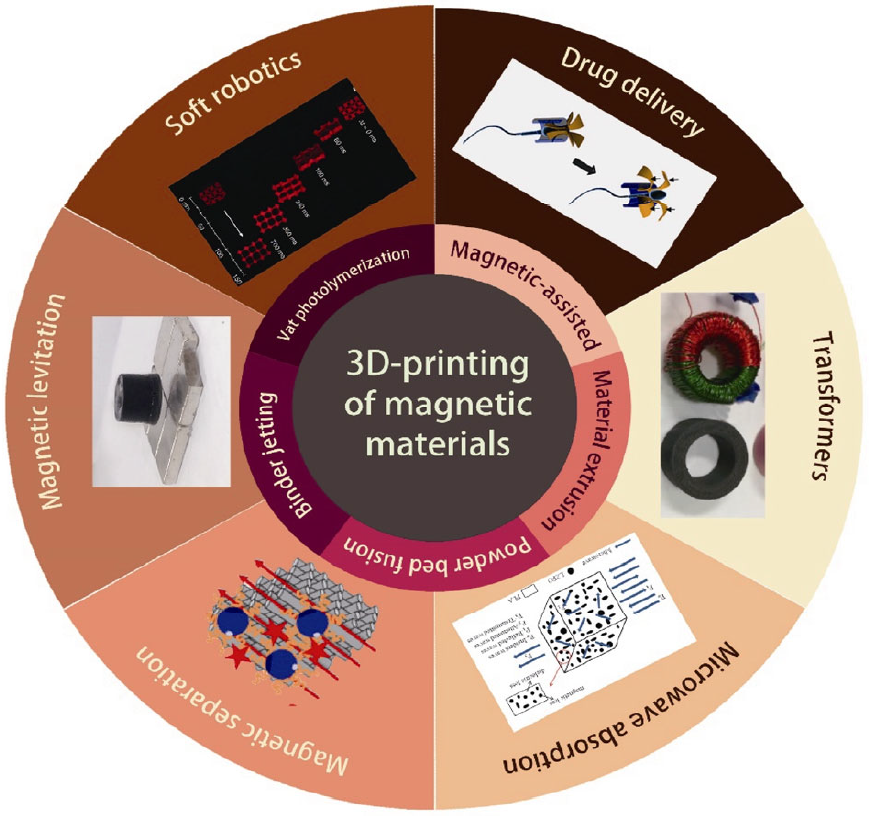
\includegraphics[width=0.5\textwidth]{images/AM_methods_and_applications.png}
\vfill

\end{frame}

\begin{frame}{Review paper - Chapter 6 - Challanges}
\begin{itemize}
    \item It is necessary to explore geometries not feasible to be achieved by state-of-the-art methods, and have unique and potentially useful magnetic functionality. 
    \item In PBF, powder properties need to be optimized and printing physics need to be studied. 
    \item In FDM and DIW, the magnetic properties are difficult to precisely control due to a tradeoff in volume fraction of the magnetic filler. 
    \item Homogeneous dispersion of magnetic fillers in the composites are a challenge.
    \item Further work could focus on in situ magnetic field alignment of particles for desired magnetic properties.
\end{itemize}
\end{frame}